%!TEX root = volumeFinal.tex 

\chapter{\label{chap:impl}Implementação}

A implementação do algoritmo de AHTN dentro do MicroRTS foi feita em duas etapas.
Primeiro foi feita a modelagem do domínio e criado qual heurística define o valor de utilidade para os estados.
Na segunda etapa foi acoplado o JSHOP2 com o MicroRTS, e logo após foi feita a implementação do algoritmo AHTN.

\section{Modelagem do domínio}

Antes de realizar a implementação do algoritmo de AHTN, é preciso criar um domínio de planejamento. 
O domínio de planejamento serve para que o JSHOP2 consiga gerar os planos que serão usados pelo algoritmo.

A modelagem do domínio inicia com a especificação de qual estratégia o domínio vai adotar.
O domínio é pensado em uma situação de jogo, onde o jogador quer treinar uma unidade de ataque para destruir o seu adversário.
Sendo assim, o jogador precisa de um quartel para treinar as unidades, e uma base para os recursos serem guardados.
O domínio tem apenas uma de cada edificação.
Apenas um \textit{worker} é utilizado, ele fica responsável pela extração dos recursos e construção das edificações.
Quando o quartel está criado, e há recursos para treinamento de um unidade de ataque, a unidade \textit{ranged} é criada.
Assim que uma unidade de ataque estiver pronta, ela é enviada para atacar o adversário.
Apenas quando a unidade \textit{ranged} é destruída que outra unidade é criada.
Todos os mapas testados iniciam com uma base, pois a base é necessária para treinar \textit{workers} e para guardar os recursos.  

A modelagem do domínio começa pela descrição dos operadores.
Cada ação que pode ser executada dentro do jogo é descrita como um operador no domínio.
Por exemplo, as ações de construir um quartel, e coletar recursos, são transformadas nos operadores $!buildbarrack$ e $!getresource$, respectivamente.
Já os métodos servem para determinar ações de mais alto nível, e devem respeitar a estratégia definida.
Por exemplo, no domínio apenas um quartel é construído, então o método deve ter uma precondição para verificar se não existe outro quartel no jogo, caso não tenha, ainda é preciso checar se há recursos suficientes para construir. 
Cada método pode encadear a chamada de outros métodos do domínio.
Isso acontece pois pode ser necessário realizar outra ação antes de conseguir realizar a ação que o método está tentando fazer.
Por exemplo, é necessário um quartel para treinar uma unidade de ataque, quando o método de treinar unidade é chamado, ele verifica que não há um quartel, e ele chama o método de construir o quartel.

Para ganhar o jogo é preciso atacar o adversário, por essa razão o método utilizado como objetivo no problema de planejamento é o $ataqueranged$.\frm{Apesar de deixar o código mesmo no apêndice, seria bom ter um diagraminha com esta estratégia.}
Esse método desencadeia todas as outras chamadas de método dependendo do estado do ambiente.
No Apêndice~\ref{ap:estra1} está a descrição deste domínio, que é chamado de domínio 1.

O domínio 1 treina apenas uma unidade de ataque, o que acaba limitando o poder de ataque da estratégia.
Para tentar solucionar esse problema, outro domínio foi modelado.
Esse domínio tem a mesma estratégia do domínio anterior, com a diferença de que mais de uma unidade de ataque é criada.
Assim, enquanto uma unidade está atacando, outra pode estar sendo treinada.
No Apêndice~\ref{ap:estra2} está a descrição deste domínio, que é chamado de domínio 2.


\section{Heurística}

O algoritmo de AHTN requer uma função de avaliação para determinar o valor de utilidade para cada estado do jogo. Essa função utiliza uma heurística para determinar o valor de utilidade.
Foram criadas duas heurísticas.
A primeira leva em consideração apenas as unidades do jogador.
Quanto maior o número de unidades disponíveis no ambiente melhor a função de avaliação do estado.
As unidades são ponderadas pelo custo de treinamento ou de construção, isso é necessário porque o custo de treinamento ou construção de cada unidade é diferente.
A Equação~\ref{eq:heu1} ilustra a formula para essa heurística.

\begin{equation}
\label{eq:heu1}	
avaliacao(s) =  (1*worker) + (5 * quartel) + (10 * base) + (2 * unidadesDeAtaque)
\end{equation}

O problema dessa heurística é que as unidades do adversário não estão sendo levadas em consideração.
Se um jogador tem o dobro de unidades que o outro, isso é um forte indicio que ele está ganhando o jogo.
Para resolver o problema outra heurística foi criada.
Essa heurística utiliza a mesma maneira de calcular da Equação~\ref{eq:heu1}, mas também calcula o mesmo valor para as unidades do adversário. 
O valor das suas unidades que o jogador possui é subtraído do valor das unidades do adversário. 
Assim em um cenário onde o jogo está com mais tropas a favor, o valor de utilidade é positivo, e caso o contrario negativo.
Esta heurística foi a escolhida para ser utilizada na implementação.

Se um jogador não tem uma base, e não tem recursos para construir uma, o jogo está perdido, pois a base é necessário para armazenar os recursos. 
Nesse caso, as duas heurísticas retornam um valor negativo, indicando o fim do jogo. 

\section{Implementação}

\subsection{Ações do MicroRTS}

Antes de iniciar a implementação do algoritmo de AHTN, é preciso criar os métodos em Java que executam as ações dentro do MicroRTS.
A camada de abstração fornece as classes que são responsáveis por exercer essas funções, mas ainda assim é preciso informar qual unidade o método está chamando.
Para isso foram criados 6 métodos que utilizam as classes da camada.
Cada método fica responsável por apenas um ação dentro do jogo.
Os métodos realizam as seguintes ações: construir uma base, construir um quartel, treinar um \textit{worker}, um \textit{worker} coleta recursos, treinar unidade de ataque, e uma unidade de ataque procura unidades adversárias para atacar.

\subsection{Geração dos planos}

O algoritmo de AHTN decompõem todas as possibilidades de plano para um objetivo com determinada configuração do jogo.
Para gerar os planos foi utilizado o planejador JSHOP2.
O JSHOP2 gera duas classes java, uma representando o domínio, e outra representando o problema.
A classe do domínio gerada traduz as informações relativas aos métodos, operadores, e as ligações entre eles, para estruturas de dados do Java.
Já a classe do problema contém o estado do ambiente e as tarefas que desejam ser alcançadas.
A classe do problema gera o plano utilizando as estruturas da classe do domínio.

A classe que representa o domínio não precisa ser alterada, pois são sempre os mesmo operadores e métodos que são utilizados para gerar o plano.
Mas o problema muda a cada nova configuração do ambiente.
Nesse caso a classe do problema deve ser alterado para que represente um novo estado.
Essa mudança foi feita alterando a classe java originada pelo JSHOP2. 
A mudança consistem em gerar novos predicados a cada nova configuração.
Para isso foi preciso uma análise de como é guardado internamente cada um dos componentes do problema de planejamento na classe do JSHOP2.
A partir dessa análise houve o mapeamento dos estados do jogo para os predicados do problema.

Uma classe chamada de $EstadoDoJogo$ foi criada para representar o estado em que o jogo está em determinado momento.
A classe contém informações das unidades que cada jogador tem em determinada configuração do jogo, podendo ser alterada caso alguma ação seja executada.
A cada novo estado é gerado um conjunto de predicados que representam o jogo, para que o planejador consiga gerar quais planos são possíveis de serem feitos.

A Figura~\ref{fig:planos} ilustra a comunicação necessária para geração dos planos.
A geração de um plano é feita a partir da chamada do método \texttt{getPlanos}.
Para isso, é necessário informar qual o estado do jogo.
A classe do problema, gerada pelo JSHOP2, pega as informações do domínio e gera os planos a partir do estado do jogo informado.
Por fim, os planos gerados são retornados para a classe dentro do MicroRTS.

\begin{figure}[ht]
	\centering
	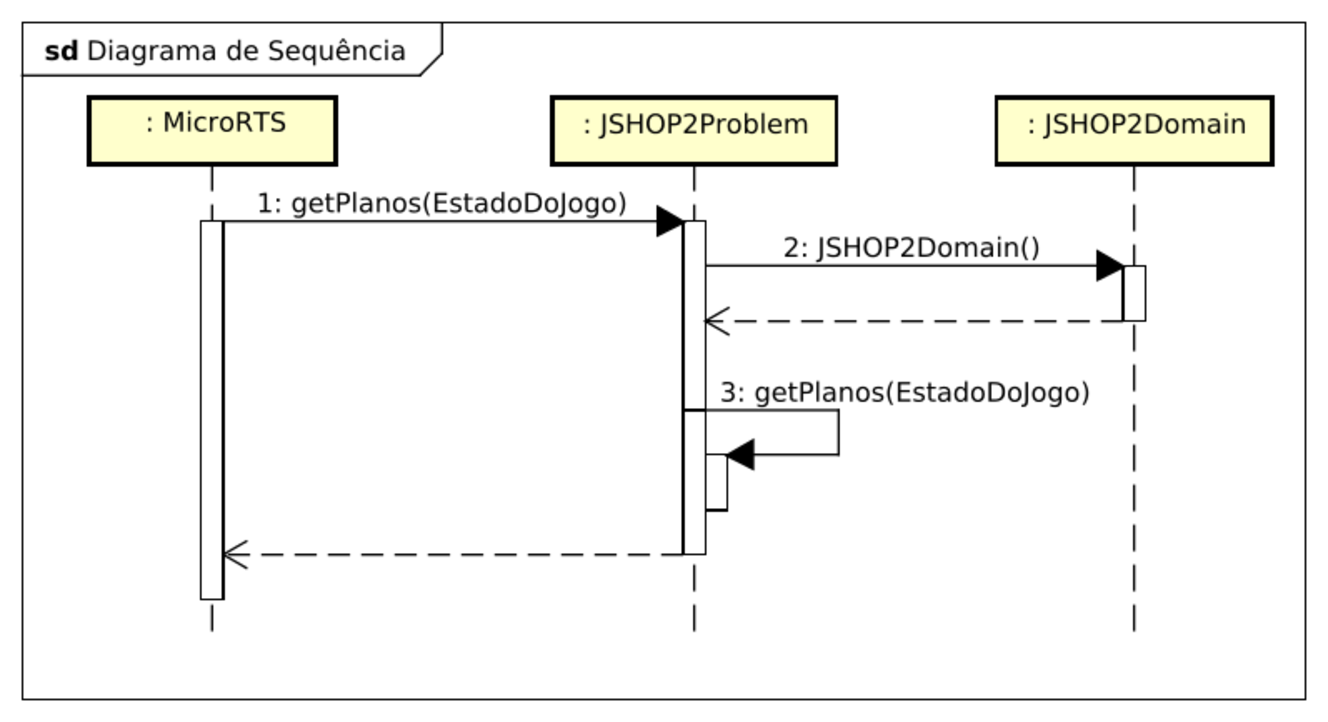
\includegraphics[width=0.9\textwidth]{fig/gerarPlano.pdf}
	\caption{Comunicação entre o MicroRTS e as classes do JSHOP2}
	\label{fig:planos}
\end{figure}

\subsection{Algoritmo de AHTN}

Para que o MicroRTS reconheça uma IA, ela deve ter o método $\mathit{getAction}$ implementado.
Quando este método é invocado a técnica deve realizar a sua operação e retornar qual movimento deve ser executado.
Sendo assim, a classe que implementa o algoritmo de AHTN deve utilizar este método para retornar a ação encontrada.
O algoritmo de AHTN implementado seguiu o padrão do algoritmo apresentado na Seção~\ref{alg:ahtn}, mas com algumas alterações.

O JSHOP2 gera os planos apenas com os operadores utilizados para alcançar o objetivo.
Com isso, o plano gerado não tem a informação de quais métodos foram utilizados para chegar aos operadores.
Neste caso, o plano contém os operadores ordenados que chegam ao objetivo.
No algoritmo de AHTN original o plano vai sendo decomposto através dos métodos a medida que a arvore das jogadas está expandindo, e só realiza a troca de perspectiva entre \textsc{Max} e \textsc{Min} quando há uma tarefa primitiva a ser executada.
No algoritmo de AHTN implementado há uma pequena diferença do algoritmo orignal.
No algoritmo implementado sempre ha troca de perspectiva a cada rodada.
A troca de perspectiva é feita para cada plano que é gerado a partir do estado do jogo.
O Algoritmo~\ref{alg:meuahtn} ilustra o pseudo código do algoritmo de AHTN implementado.

O algoritmo recebe um estado, representando qual a configuração do ambiente, um plano para a perspectiva \textsc{Max}, um plano para a perspectiva \textsc{Min}, e uma profundidade.
A Linha~\ref{alg:meuahtn:terminal} verifica se o estado é uma configuração de final de jogo, ou ainda se a profundidade configurada não chegou ao fim.
Caso uma das duas coisas aconteça, o algoritmo retorna o plano de cada perspectiva, e também a função de avaliação para a configuração em que o jogo se encontra.

O algoritmo avança caso não haja uma configuração de final de jogo.
Na linha~\ref{alg:meuahtn:nexaction} o algoritmo aplica a próxima ação primitiva do plano no estado.
Neste ponto, o jogador, na perspectiva do \textsc{Max}, realiza uma ação no estado.
Após alterar o estado, o algoritmo gera todos os planos para \textsc{Min} a partir do novo estado, e realiza a chamada para o método $\mathit{AHTNMin}$.
O método de $\mathit{AHTNMin}$ realiza as mesmas operações que o método de $\mathit{AHTNMax}$ mas com a perspectiva de \textsc{Min}.
Seguindo, na linha~\ref{alg:meuahtn:avali}, o algoritmo verifica qual dos planos obteve a melhor função de avaliação. 
Com isso, o algoritmo decide qual a melhor opção de plano.
O melhor plano é retornado na linha~\ref{alg:meuahtn:retorno}.


\begin{algorithm}[ht]
	\caption{Pseudo código do algoritmo de AHTN implementado.}
	\label{alg:meuahtn}
 	\begin{algorithmic}[1]		
 		\Function {ATHNMax}{$estado, planoMax, planoMin, deph$}
	 		\If {$terminal(estado) \vee d \leq 0$} \label{alg:meuahtn:terminal}
		 		\State	\Return $(planoMax, planoMin, avaliacao(estado))$
	 		\EndIf
	 		\State {$nextAction(planoMax)$} \label{alg:meuahtn:nexaction}
	 		\State $(Pmax', Pmin', ev') = \perp, \perp, -\infty$
			\ForAll{$plano \in getPlanosMin(estadoDoJogo)$} \label{alg:meuahtn:for}
		 		\State $(Pmax, Pmin, ev) = \Call{AHTNMin}{(estado, planoMax, planoMin, deph-1)}$ \label{alg:meuahtn:ahtnmin}
			 	\If {$ev' > ev$} \label{alg:meuahtn:avali}
					\State $(Pmax', Pmin', ev') = (Pmax, Pmin, ev)$
				\EndIf		 		 		
		 	\EndFor
		 	\State \Return $(Pmax', Pmin', ev')$ \label{alg:meuahtn:retorno}
 		\EndFunction
 	\end{algorithmic}
 \end{algorithm}
 
 
O método $\mathit{getAction}$ é responsável pela chamada do algoritmo de AHTN. 
Ele realiza a chamada para o método de $\mathit{AHTNMax}$ para todos os planos possíveis no estado atual.
O retorno indica qual plano tem a melhor função de avaliação.
A primeira ação do plano com a melhor função de avaliação é a escolhida para ser executada. 

O método $\mathit{getAction}$ é chamado a todo o ciclo para decidir qual a jogada deve ser realizada.
As ações geralmente não são realizadas em um clico.
Por exemplo, treinar uma unidade leva alguns ciclos.
Assim o algoritmo gera muitas vezes a mesma ação.
Foi definido um tempo de 50 ciclos para gerar uma nova ação.
Com isso o número de ações geradas repetidamente foi reduzido.

